\documentclass{beamer}

\usepackage{hyperref}
\usepackage{amsmath}
\usepackage{amsfonts}
\usepackage[ruled]{algorithm}
\usepackage{algpseudocode}
\usepackage{graphicx}
\usepackage{minted}

\newcommand {\I} {\ensuremath {\mathbf{1\hspace{-5.5pt}1}}}
\renewcommand{\vec}[1]{\ensuremath{\boldsymbol{#1}}}

\title{Design and Implementation of\\Anglican Probabilistic Programming Language}
\author{David Tolpin \and Jan Willem van de Meent \and Hongseok Yang \and Frank Wood}
  
\AtBeginSection[]
{
  \begin{frame}<beamer>
    \frametitle{Outline}
    \tableofcontents[currentsection]
  \end{frame}
}

\begin{document}


\begin{frame}
\titlepage
\vfill
\center
Paper and slides: \url{https://bitbucket.org/probprog/anglican-white-paper}

\end{frame}

\section{Why probabilistic programming?}

\begin{frame}{Intuition}
    \textbf{Probabilistic program:}
\begin{itemize}
\item A program with random computations.
\item Distributions are conditioned by `observations'.
\item Values of certain expressions are `predicted' --- \textbf{the output}.
\end{itemize}

Can be written in any language (extended by \texttt{sample} and \texttt{observe}).
\end{frame}

\begin{frame}[fragile]{Example: Model Selection}
\begin{minted}[linenos, fontsize=\small]{clojure}
(let [;; Guessing a distribution
      dist (sample (categorical
                     [[normal 1] [gamma 1]
                      [uniform-continuous 1]
                      [uniform-discrete 1]]))
      a (sample (gamma 1 1))
      b (sample (gamma 1 1))
      d (dist a b)]

  ;; Observing samples from the distribution
  (loop [data data]
    (when (seq data)
      (let [[x & data] data]
        (observe d x))
      (recur data)))

  ;; Predicting a, b and the distribution
  (predict :a a) 
  (predict :b b)
  (predict :d d))
\end{minted}
\end{frame}

\begin{frame}{Definition}

A \textbf{probabilistic program} is a stateful deterministic
computation $\mathcal{P}$:
\pause
\begin{itemize}
\item Initially, $\mathcal{P}$ expects no arguments.
    \pause
\item On every call, $\mathcal{P}$ returns
    \begin{itemize}
        \item a distribution $F$,
        \item a distribution and a value $(G, y)$,
        \item a value $z$, 
        \item or $\bot$.
    \end{itemize}
    \pause
\item Upon returning $F$, $\mathcal{P}$ expects $x\sim F$.
    \pause
\item Upon returning $\bot$, $\mathcal{P}$ terminates.
\end{itemize}
\pause
A program is run by calling $\mathcal{P}$ repeatedly until termination.

The probability of each \textbf{trace} is $\propto\prod_{i=1}^{\left|\pmb{x}\right|} p_{F_i}(x_i) \prod_{j=1}^{\left|\pmb{y}\right|}p_{G_j}(y_{j})$.
\end{frame}

\begin{frame}{Evolution of Compiler Development}
    \begin{itemize} 
        \item 1950s: Ask a programmer to implement an algorithm efficiently: They'll write it on their own in assembly.
            \begin{itemize}
                \item   No good compilers; problem-dependent optimizations that only human expert could see.
            \end{itemize}
            \pause
        \item   1970s: Novice programmers use high-level languages and let compiler work out details, experts still write assembly.
            \begin{itemize}
                \item   Experts still write custom assembly when speed critical.
            \end{itemize}
            \pause
        \item   2000s: On most problems, even experts can't write faster assembly than optimizing compilers.
            \begin{itemize}
                \item   can automatically profile (JIT).
                \item   can take advantage of paralellization, complicated hardware, make appropriate choices w.r.t. caching.
                \item   Compilers embody decades of compiler research
            \end{itemize}
    \end{itemize}
\end{frame}

\begin{frame}{Evolution of Inference}

    \begin{itemize}
\item           2010: Ask a grad student to implement inference efficiently: They'll write it on their own.
    \begin{itemize}
\item   No good automatic inference engines; problem-dependent optimizations that only human expert can see.
    \end{itemize}
    \pause
\item   2015: Novice grad students use automatic inference engines and let compiler work out details, experts still write their own inference.
    \begin{itemize}
\item   Experts still write custom inference when speed critical.
    \end{itemize}
    \pause
\item   2020: On most problems, even experts can't write faster inference than mature automatic inference engines.
    \begin{itemize}
\item   Can use paralellization, sophisticated hardware
\item   Can automatically choose appropriate methods (meta-reasoning?).
\item   Inference engines will embody 1 decade (!) of PP research.
    \end{itemize}
    \end{itemize}
\end{frame}

\section{Why functional?}

\begin{frame}{Inference Objective}
\begin{itemize}
\item Suggest \textbf{most probable explanation} (MPE) - most likely assignment
  for all non-evidence variable given evidence.
  \pause
\item Approximately \textbf{compute integral} of the
  form $$\Phi=\int_{-\infty}^{\infty} \varphi(x)p(x) dx$$
  \pause
\item Continuously and \textbf{infinitely generate a sequence of samples} drawn
  from the distribution of the output expression --- so that someone
  else puts it in good use (vague but common). $\checkmark$
\end{itemize}
\end{frame}

\begin{frame}{Example: Inference Results}
  \begin{figure}[H]
      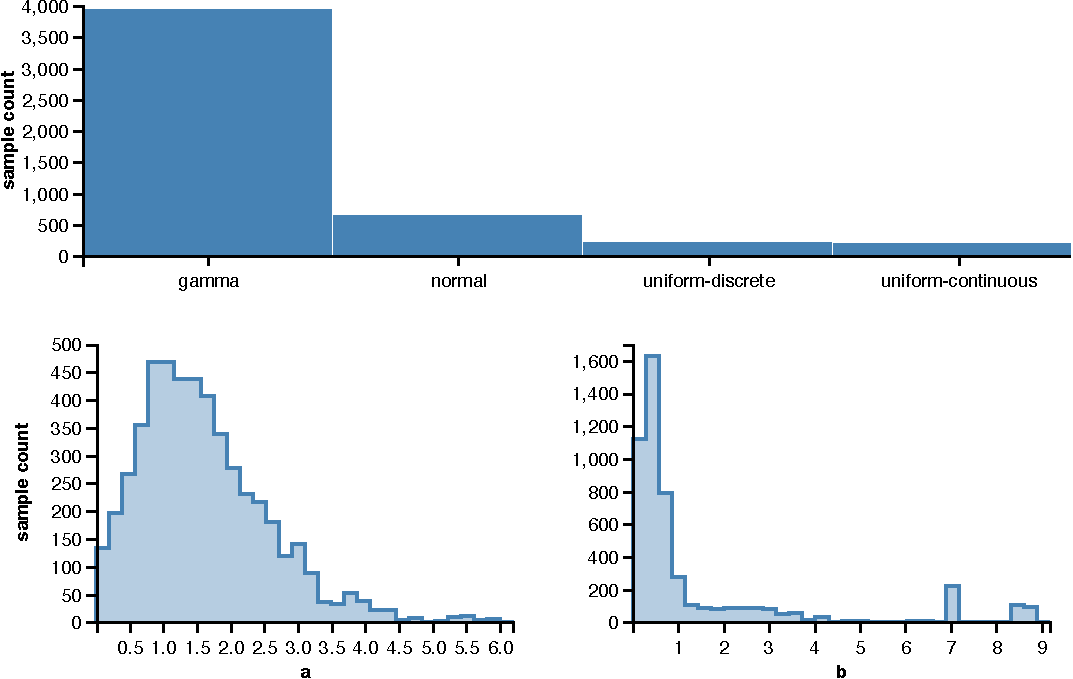
\includegraphics[scale=0.6]{models-results.pdf}
  \end{figure}
\end{frame}

\begin{frame}{Importance Sampling}
    \begin{algorithmic}
        \Loop
            \State Run $\mathcal{P}$, computing weight $w=\prod_{j=1}^{\left|\pmb{y}\right|}p_{G_j}(y_{j})$.
            \State output $\pmb{z}, w$.
        \EndLoop
    \end{algorithmic}
    \begin{itemize}
        \item[] 
         \item Simple --- good.
         \item Slow convergence (unless one knows the answer) --- bad.
     \end{itemize}
     \vfill
     Can we do better?
\end{frame}

\begin{frame}{Lightweight Metropolis-Hastings (LMH)}
\begin{algorithmic}
    \State {Run $\mathcal{P}$ once, remember $\pmb{x}, \pmb{z}$.}
    \Loop
         \State {Uniformly select $x_i$}.
         \State {Propose a value for $x_i$.}
         \State {Run $\mathcal{P}$, remember $\pmb{x'}, \pmb{z'}$}.
         \State {Accept ($\pmb{x,z}=\pmb{x',z'}$) or reject with MH probability}.
         \State {Output $\pmb{z}$.}
    \EndLoop
\end{algorithmic}
\vfill
Can we do better?
\begin{itemize}
    \item Particle Markov Chain Monte Carlo
    \item Variational Inference
    \item ...

\end{itemize}
\end{frame}

\begin{frame}{Challenges}
    \begin{itemize}
        \item `Transformational compilation' --- limited languages, some less ugly than others.
        \item Slow inference --- Markov Chain Monte Carlo is \textbf{always slow} (but there are Hybrid Monte Carlo, Variational Inference, ...)
        \item How to learn persistently --- what is the learned model? Transfer learning?
        \item Handling indeterminism (learning policies).
    \end{itemize}
\end{frame}

\begin{frame}
    \LARGE
    \center
    Thank you!\\Questions?
\end{frame}




\end{document}
